\documentclass{amsart}
\usepackage{amsmath,amsthm,amssymb,bm}
\usepackage{graphicx,color}
\usepackage{tikz}
\usepackage[T1]{fontenc}

\begin{document}

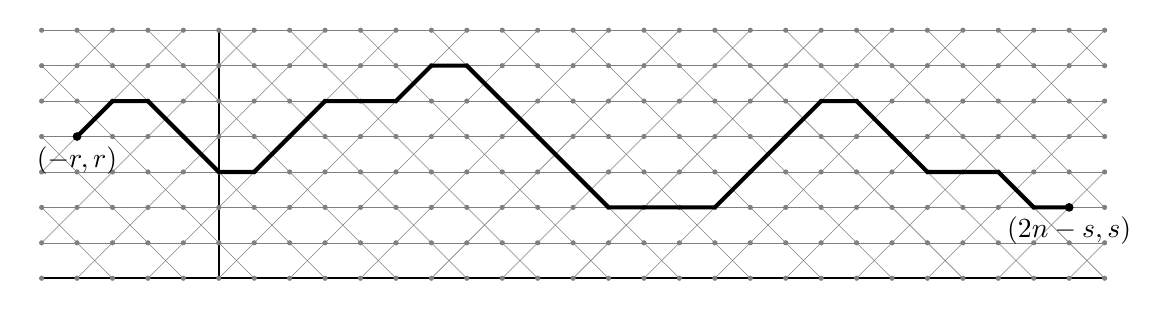
\begin{tikzpicture}[scale = 0.45]
  \foreach \y in {0,1,...,7}{\draw[help lines] (-5,\y)--(25,\y);}
  \draw[help lines] (-5,1)--(1,7) (-5,3)--(-1,7) (-5,5)--(-3,7) (20,0)--(25,5) (22,0)--(25,3) (24,0)--(25,1);
  \draw[help lines] (-5,6)--(1,0) (-5,4)--(-1,0) (-5,2)--(-3,0) (20,7)--(25,2) (22,7)--(25,4) (24,7)--(25,6);
  \foreach \x in {-4,-2,...,18}{\draw[help lines] (\x,0)--(\x+7,7);}
  \foreach \x in {-4,-2,...,18}{\draw[help lines] (\x,7)--(\x+7,0);}
  \draw[line width = 0.8pt] (0,0)--(0,7);
  \draw[line width = 0.8pt] (-5,0)--(25,0);
  \foreach \x in {-5,-4,...,25}{
    \foreach \y in {0,1,...,7}{
      \filldraw[gray] (\x,\y) circle (1.6pt);
    }}
  \filldraw[black] (-4,4) circle (3pt) node[below]{\( (-r,r) \)};
  \filldraw[black] (24,2) circle (3pt) node[below]{\( (2n-s,s) \)};
  \draw[line width = 1.5pt] (-4,4) -- ++(1,1) -- ++(1,0) -- ++(1,-1) -- ++(1,-1) -- ++(1,0) -- ++(1,1) -- ++(1,1) -- ++(1,0) -- ++(1,0) -- ++(1,1) -- ++(1,0) -- ++(1,-1) -- ++(1,-1) -- ++(1,-1) -- ++(1,-1) -- ++(1,0) -- ++(1,0) -- ++(1,0) -- ++(1,1) -- ++(1,1) -- ++(1,1) -- ++(1,0) -- ++(1,-1) -- ++(1,-1) -- ++(1,0) -- ++(1,0) -- ++(1,-1) -- ++(1,0);
\end{tikzpicture}

\end{document}